\scanpage{136}
que $G\mathrm{x}V\handwritten{\longrightarrow}V\mathrm{x}V$ est un monomorphisme (c'est le lemme de Nakayama), et on sait bien alors (SGA 3 $\mathrm{VII}_{\mathrm{B}}$ ...) que \deleted{$V$ est un} l'on a un joli quotient $W=V/G$, avec $\deleted{W\quad V}$ $V\handwritten{\longrightarrow}W$ plat et en fait la projection structurale d'un $G_{W}$-torseur. Bien sûr la coalgèbre $\overset{\handwritten{-}}{M}$ n'est autre que celle qui définit le quotient $W$ précédent. En général, il n'est pas question de prouver que $V\handwritten{\simeq}W\mathrm{x}G$ comme variété formelle à opérateurs (i.e. que le torseur précédent est trivial), i.e. de trouver une\deleted{isomorphisme} section de $V$ sur $W$, i.e. un relèvement de comodules $\overset{\handwritten{-}}{M}\handwritten{\longrightarrow}M$; on peut seulement dire que tout relèvement en tant que $k$-vectoriels définira un isomorphisme $A\otimes_{k}\overset{\handwritten{-}}{M}\handwritten{\simeq}M$ de $A$-modules. Cependant, si $G$ est formellement lisse i.e. le dual de $A$ une algèbre de \rlap{p}séries formelles (éventuellement à un nb infini de générateurs) alors on aura splittage parfait; ce sera la cas en particulier en car. nulle.

\uline{Exemple} 2. Supposons $A$ commutative pour sa loi d'algèbre. Donc $A$ est l'algèbre affine d'un schéma en monoïdes 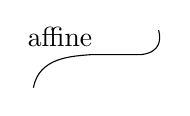
\begin{tikzpicture}[baseline=-.6ex,x=1cm,y=1cm]
\node[anchor=west,inner sep=0] at (0,.42) {\inserted{affine}};
\draw (.08,-.22) .. controls (.15,.16) and (.55,.18) .. (.82,.2) -- (1.45,.2) .. controls (1.7,.23) and (1.7,.4) .. (1.67,.51);
\end{tikzpicture} $G$. L'hypothèse sur la filtration coc\deleted{c}omplète est assez étrange ici, elle s'énonce en disant que pour toute $f\handwritten{\in}A$ (fonction sur $G$) \deleted{nulle en $e$}, il existe un entier $n$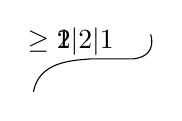
\begin{tikzpicture}[baseline=-.6ex,x=1cm,y=1cm]
\node[anchor=west,inner sep=0] at (0,.42) {\inserted{$\handwritten{\geq\unsure{\rlap{\(1\)}2|2|1}}$}};
\draw (.08,-.22) .. controls (.15,.16) and (.55,.18) .. (.82,.2) -- (1.35,.2) .. controls (1.6,.23) and (1.6,.4) .. (1.57,.51);
\end{tikzpicture} tel que la fonction en $n$\deleted{\unsure{s|x}} variables $f(g_{1}g_{2}\cdots g_{n})$ soit \deleted{identiquement nulle}\inserted{somme de fonctions} à $n-1$ parmi les var\rlap{a}i\rlap{a}ibles.\margin{\figure{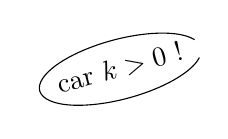
\begin{tikzpicture}[rotate=15,transform shape]
\node[inner sep=3pt] (n) {\handwritten{car $k>0$ !}};
\draw (1.01,.10) arc[start angle=18,end angle=342,x radius=1.06cm,y radius=.38cm];
\end{tikzpicture}}} Si $G$ est de type fini sur $k$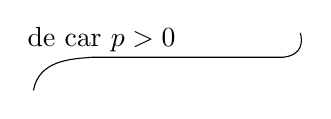
\begin{tikzpicture}[baseline=-.6ex,x=1cm,y=1cm]
\node[anchor=west,inner sep=0] at (0,.42) {\inserted{\handwritten{de car $p>0$}}};
\draw (.08,-.22) .. controls (.15,.16) and (.55,.18) .. (.82,.2) -- (3.25,.2) .. controls (3.5,.23) and (3.5,.4) .. (3.47,.51);
\end{tikzpicture}, je pense que \deleted{dès qu'on y remplace une des variables par $1$, mais alors, faisant tous} cela doit entrai\rlap{t}ner que \deleted{l'unité de} $G$ est \figure{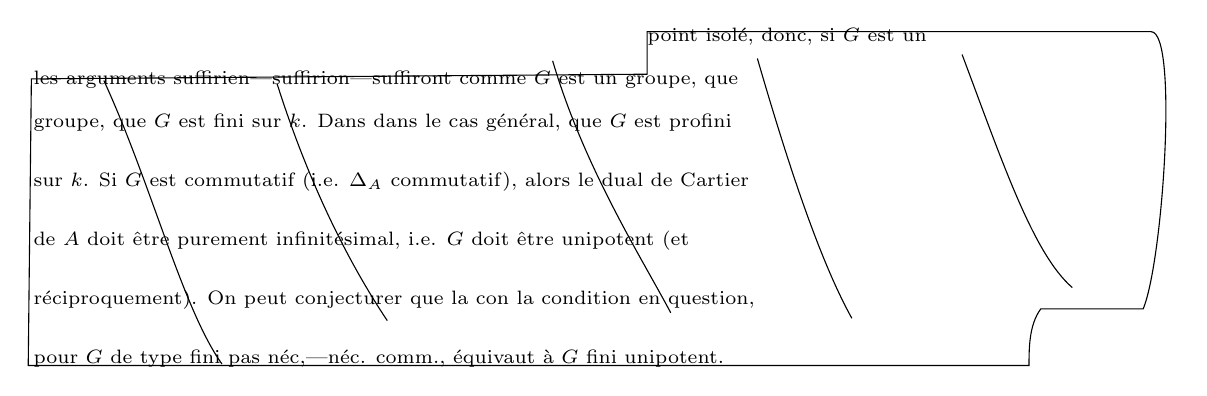
\begin{tikzpicture}[x=1cm,y=1cm,every node/.style={anchor=base west,inner sep=0,font=\scriptsize}]
\node at (7.8,0) {\deleted{point isolé, donc, \deleted{si $G$ est un}}};
\node at (0,-0.55) {\deleted{\deleted{les arguments \unsure{suffirien|suffirion|suffiront}} comme $G$ est un groupe, que}};
\node at (0,-1.1) {\deleted{\deleted{groupe, que} $G$ est fini sur $k$. \deleted{Dans dans le cas général, que $G$ est profini}}};
\node at (0,-1.85) {\deleted{\deleted{sur $k$.} Si $G$ est commutatif (i.e. $\handwritten{\Delta}_{A}$ commutatif), alors le dual de Cartier}};
\node at (0,-2.6) {\deleted{de $A$ doit être purement infinitésimal, i.e. $G$ doit être unipotent (et}};
\node at (0,-3.35) {\deleted{réciproquement). On peut conjecturer que \deleted{la con} la condition en question,}};
\node at (0,-4.1) {\deleted{pour $G$ de type fini pas \unsure{néc,|néc.} comm., équivaut à $G$ fini unipotent.}};
\draw (7.8,.12) -- (14.2,.12) .. controls (14.55,.12) and (14.35,-2.8) .. (14.1,-3.4) -- (12.8,-3.4) .. controls (12.65,-3.6) and (12.65,-3.9) .. (12.65,-4.12) -- (-.06,-4.12) -- (-.02,-.48) -- (7.8,-.42) -- cycle;
\draw (.9,-.50) .. controls (1.5,-1.8) and (1.9,-3.4) .. (2.4,-4.10);
\draw (3.1,-.54) .. controls (3.5,-1.8) and (4.0,-2.8) .. (4.5,-3.55);
\draw (6.6,-.25) .. controls (7.0,-1.6) and (7.7,-2.7) .. (8.1,-3.45);
\draw (9.2,-.22) .. controls (9.6,-1.6) and (10.0,-2.8) .. (10.4,-3.52);
\draw (11.8,-.17) .. controls (12.3,-1.5) and (12.7,-2.7) .. (13.2,-3.13);
\end{tikzpicture}}\margin{\handwritten{?}}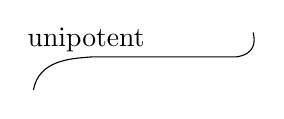
\begin{tikzpicture}[baseline=-.6ex,x=1cm,y=1cm]
\node[anchor=west,inner sep=0] at (0,.42) {\inserted{\handwritten{unipotent}}};
\draw (.08,-.22) .. controls (.15,.16) and (.55,.18) .. (.82,.2) -- (2.65,.2) .. controls (2.9,.23) and (2.9,.4) .. (2.87,.51);
\end{tikzpicture} donc si on ne suppose plus non plus $G$ de type fini, que $G$ est \deleted{profini et} prounipotent.

% archive sheet number: 135
